\chapter{The CMS Experiment}

In the previous chapter we summarized the theoretical underpinnings of modern
particle physics, and discussed possible extensions that point towards
future research. We now turn our attention to the machines that make such
research possible. The Large Hadron Collider (LHC) is the largest
particle collider ever built, smashing protons together at record energies.
On it are located four major experiments, designed to record electrical
snapshots of the collisions and allow physicists to reconstruct the details
of each event. Sec.~\ref{sec:lhc} describes the design and operation of the LHC,
and Sec.~\ref{sec:cms_det} introduces the Compact Muon Solenoid (CMS) experiment,
one of the four at the LHC and the one used for the analysis in this dissertation.

\section{The Large Hadron Collider}
\label{sec:lhc}

Underneath the Franco-Swiss border near the city of Geneva lies the LHC, the world's largest 
proton collider. With a circumference of 26.7 kilometers and depth of up to 175
meters below ground, it is designed to accelerate protons to an energy of 7\TeV, over
7,000 times their rest mass (and corresponding to a speed 
99.9999991\% the speed of light). Utilizing the tunnel of the older Large Electron--Positron
collider (LEP) at CERN, it was constructed to supersede the Tevatron at Fermilab, which
accelerated protons to 1\TeV.

What was the motivation for such a machine? The LEP collider, which accelerated electrons
and positrons to up to 209\GeV, had allowed for precise measurements of many SM quantities
inclusing the $W$ and $Z$ masses, but was not able to find definitive proof of a Higgs boson
or any evidence for BSM physics. Similarly, the Tevatron had discovered the top quark
and made many measurements but failed to find evidence of the Higgs or new physics. Physicists
thus sought a next-generation machine that could find these things.

\begin{figure}[t]
  \begin{center}
    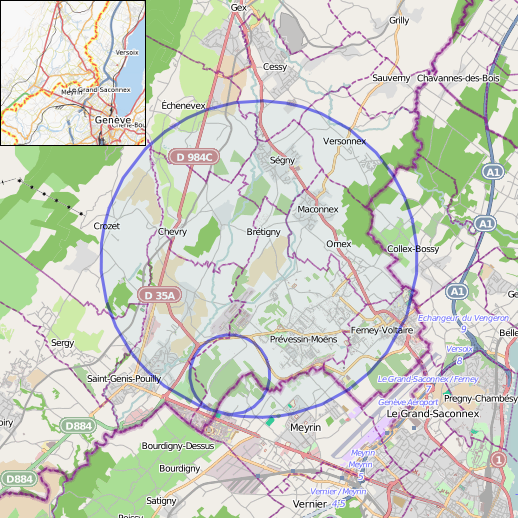
\includegraphics[width=0.39\textwidth]{figs/cms/lhc_osm.png}
    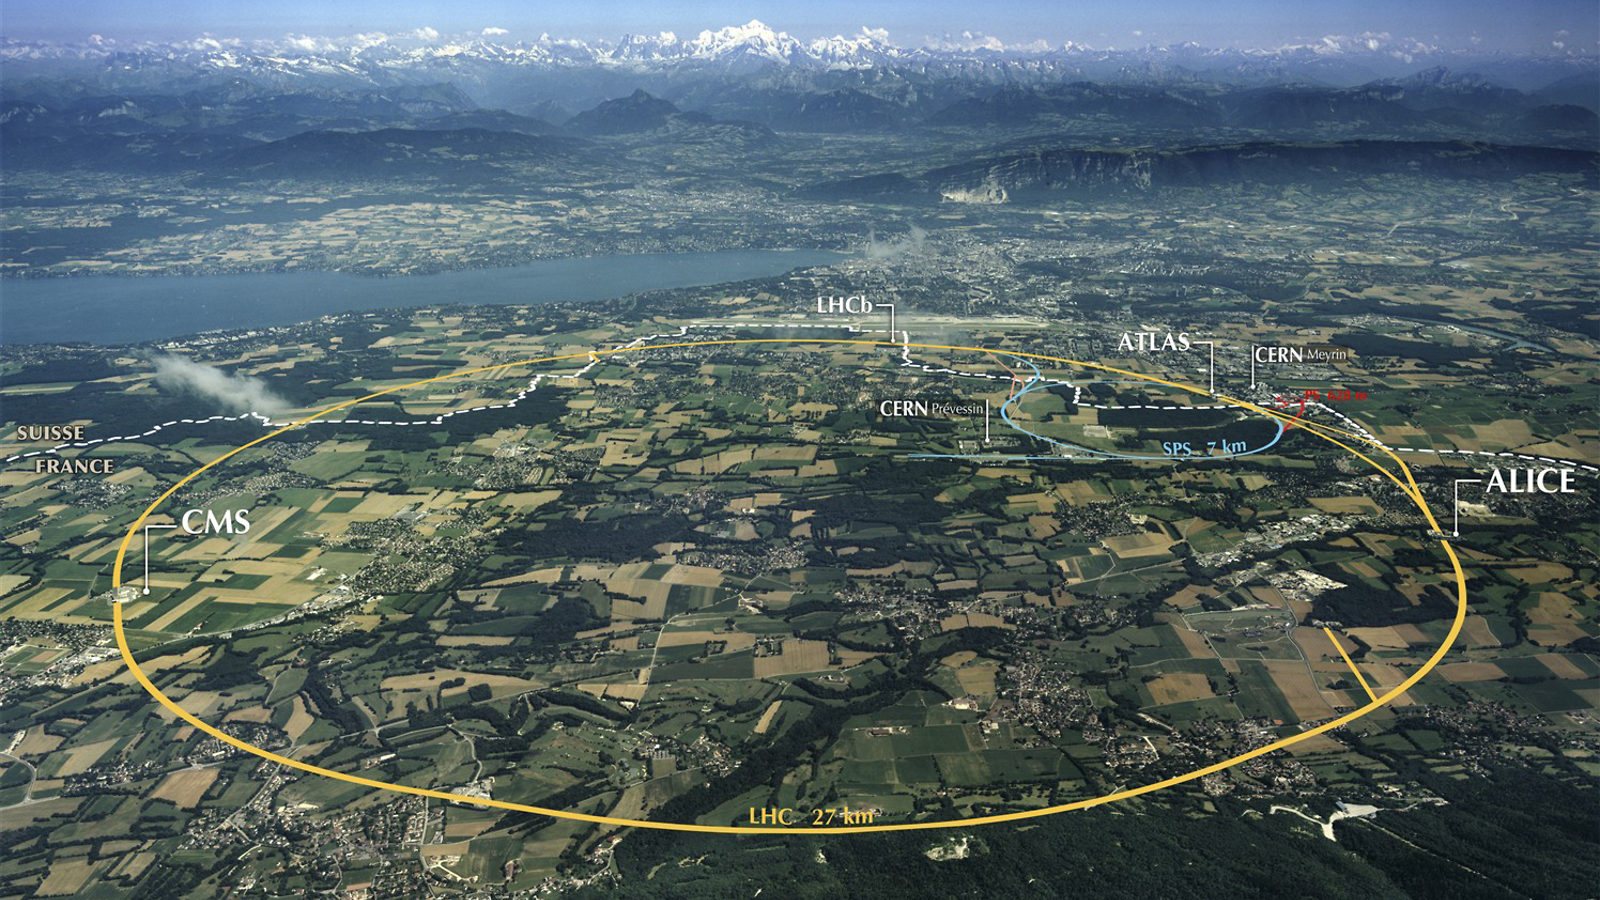
\includegraphics[width=0.59\textwidth]{figs/cms/lhc_photo.jpg} 
    \caption{(left) The SPS and LHC overlaid on a map of the Franco-Swiss border near Geneva. The diameter of
      the LHC is 8.5 km (5.3 miles). (right) The LHC, the four major experiments, and CERN's campus 
      overlaid on a photo of the Geneva area, looking southeast. Lake Geneva and the French Alps can
      be seen in the background. (Images from \cite{lhc_map,lhc_photo})
            }
    \label{fig:lhc}
  \end{center}
\end{figure}

Since the Higgs and potential new physics were at energy scales above the reach of
current experiments, a higher energy collider was needed. 
Circular lepton colliders like LEP
are limited in energy, as the energy radiated by an accelerating charged particle falls as 
$1/m^4r^2$, and so the size of the necessary electron collider would be prohibitive.
The much heavier proton is far easier to accelerate to high energies, and an accelerator
in the pre-existing LEP tunnel was sufficient to achieve the necessary energies
(and additionally, cost-effective).
The downside is that collisions of composite particles like protons are messy, and
the actual parton collision energy is indeterminate. However, the LHC was meant do be a 
``discovery machine'', so probing a wide range of collision energies was desirable.
For precision studies of any interesting physics uncovered by the LHC, a future
linear $e^+e^-$ collider would be a good option.

From these considerations, the particle physics community 
decided on a $pp$ collider built in the LEP tunnel,
and construction on the LHC began in 1998. A map of its location can be seen in
Fig.~\ref{fig:lhc}. It sits in a tunnel between 50 and 175 meters underneath
the suburbs of Geneva, Switzerland, straddling the France-Switzerland border.
To the west are the Jura mountains, and to the east Lake Geneva. The CERN
campus is on the south end.

\begin{figure}[t]
  \begin{center}
    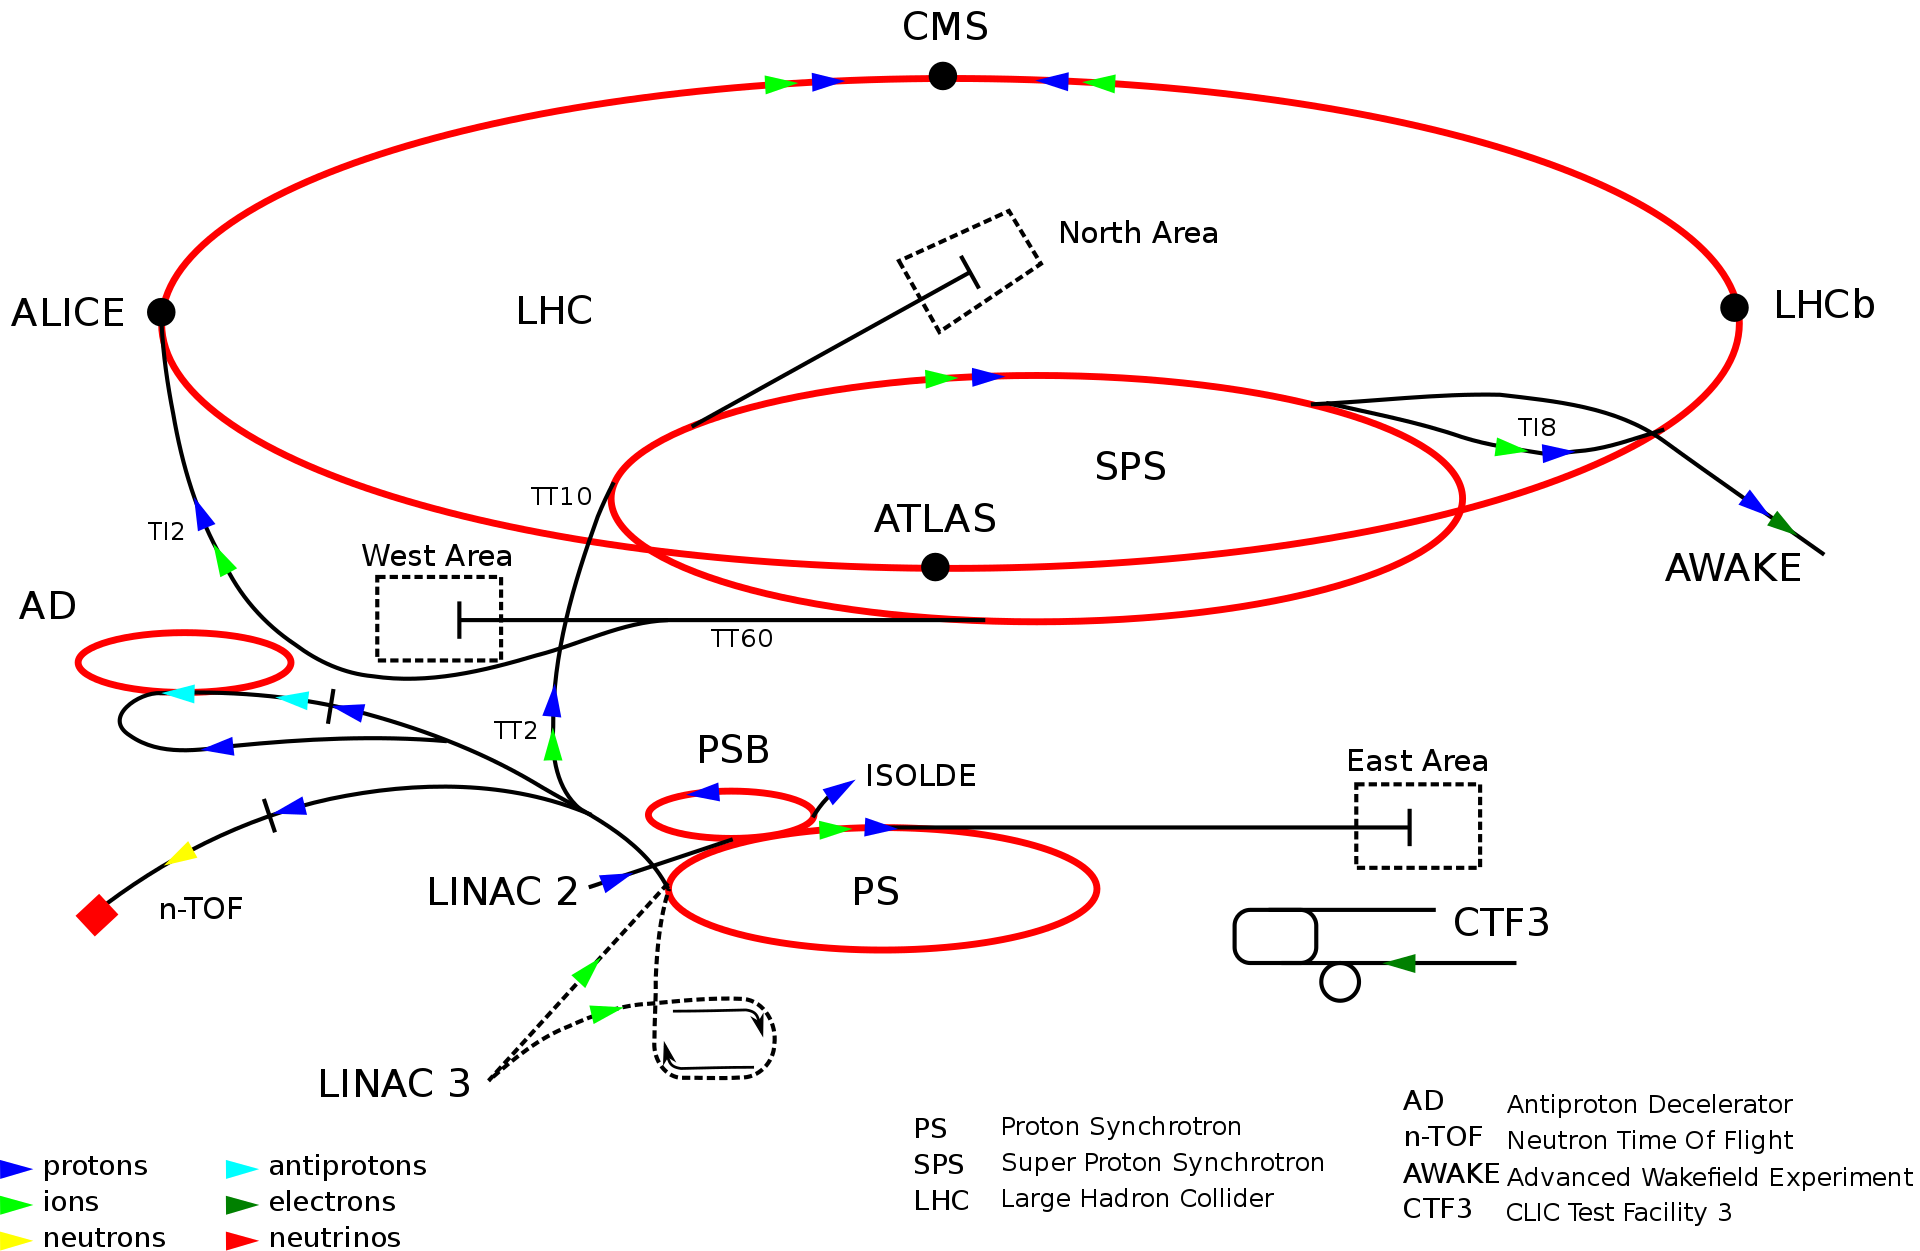
\includegraphics[width=0.60\textwidth]{figs/cms/accelerator_complex.png}
    \caption{The CERN accelerator complex. Protons originate in the LINAC 2 where they are 
      injected at 50\MeV into the PSB. The PSB, PS, and SPS subsequently accelerate them
      to 1.4\GeV, 26\GeV, and 450\GeV, respectively, before they enter the LHC where they
      reach up to 6.5\TeV. (Image from~\cite{accelerator_complex})
            }
    \label{fig:cern_accelerator_complex}
  \end{center}
\end{figure}

Before being injected into the main ring, the protons progress through a series of
increasingly large accelerators. The steps in the chain are as follows;
the CERN accelerator complex is
illustrated in Fig.~\ref{fig:cern_accelerator_complex}. 
\begin{itemize}\setlength\itemsep{-1mm}
\item The protons begin as nuclei in hydrogren gas, and electric fields are used to strip the electrons away.
\item The bare protons are fed into the linear LINAC 2 accelerator, where
they are boosted to 50\MeV kinetic energy and injected into the 160 meter
Proton Synchrotron Booster (PSB).
\item The PSB accelerates the protons to 1.4\GeV and feeds them into the
628 meter Proton Synchrotron (PS).
\item The PS accelerates them to 26\GeV and injects them into the
6.9 kilometer Super Proton Synchrotron (SPS).
\item The SPS accelerates them to 450\GeV before finally injecting
them into the main 26.7 kilometer LHC ring (it inserts two beams, traveling
in opposite directions)
\item Over a period of around 20 minutes, the LHC accelerates the protons
to 6.5\TeV (this is the present maximum; the LHC is designed to eventually
go to 7\TeV).
\end{itemize}

In order to steer the beams in a circle, the LHC makes use of powerful superconducting
magnets. Dipole magnets are used as the main steering mechanism. From the formula 
for a relativistic charged particle in a uniform magnetic field, the necessary average
magnetic field is $B=\gamma m\beta/qR=5.1~\mrm{T}$. However, the magnets are not all the
way around the ring so the peak dipole magnetic field is 7.74 T. In addition to the dipole magnets,
quadrupole magnets are used for beam focusing, and higher multipole magnets are used for finer
corrections. In total there are nearly 10,000 individual magnets. In order to maintain a such a
strong field, the superconducting magnets operate at a temperature of only 1.9 K, achieved
using 96 tons of superfluid helium~\cite{lhc_guide}.

Magnets can only steer the beam, not increase its energy. In order to perform
the acceleration from 450\GeV to 6.5\TeV, the LHC makes use of 8 radio-frequency
(RF) cavities per direction that produce an oscillating electric field at a frequency of
400 MHz. This naturally produces a beam of ``bunches'', spaced 25 ns apart:
the electric fields boost the protons, and the gradient of the field is
constructed in such a way that any protons that arrive early or late
recieve a slightly different kick, pushing them back towards the bunch
center.

Together, the magnetic and electric fields produce two counter-rotating
beams of 6.5\TeV protons, organized into bunches 25 ns apart. There are around
$1.2\times10^{11}$ protons per bunch, and up to 2808 bunches per beam, giving
$3.4\times10^{14}$ protons in each beam. At 6.5\TeV each, the total kinetic energy
in both beams together is over 700 million joules, equivalent
to a Boeing 737 traveling at 200 mph!

The ``collision rate'' at colliders is measured with a quantity known as instantaneous
luminosity, defined by the rate $N$ of a given type of interaction with cross section (roughly, likelihood
of interaction) $\sigma$ as $\mathcal{L}=N\sigma$. This luminosity is a function of
the bunch crossing rate (at the LHC, once every 25 ns), the number of protons
per bunch, and the effective area of the beam (i.e., how tightly packed
the protons in the beam are). The LHC can reach an instantaneous luminosity of
around $2\times10^{34}~\mrm{cm}^{-2}\mrm{s}^{-1}$.

The total proton-proton inelastic cross section is measured to be around 78 mb~\cite{ATLAS:ppxsec}.
Multiplying by the LHC instantaneous luminosity, that means we expect
1.5 billion inelastic collisions per second, or around 40 per bunch crossing.
Most of these will be relatively uninteresting, and a major challenge in analyzing experimental
data is disentagling the interesting event from the $\sim40$ other interactions
(referred to as \textit{pileup} interactions).

% collision points and experiments
The LHC steers the counter-rotating beams to collide at four pre-defined
experimental interaction points, corresponding to the ATLAS, ALICE,
CMS, and LHCb experiments (illustrated in Figs.~\ref{fig:lhc} (right)
and \ref{fig:cern_accelerator_complex}). 
We now turn our attention to one of these in particular: the CMS experiment.


\section{The CMS detector}
\label{sec:cms_det}

\section{Phase-2 CMS MIP timing detector}
